\section{二面体群与自由群}


参考：[DF] Dummit–Foote《Abstract Algebra》§1.2（二面体群）、§6.3（自由群）；[DS]《离散数学与结构》§9.1、§9.3。

记号说明：采用 [DF] 的 $D_{2n}$（下标是群的阶）；[DS] 把同一个群记作 $D_n$。

\subsection{二面体群}


正 $n$ 边形（$n\ge3$）的全体对称在复合下构成二面体群（dihedral group）$D_{2n}$，共有 $2n$ 个元素。取 $r$ 为旋转 $2\pi/n$，$s$ 为一条固定轴的反射，则

\[r^n=e,\qquad s^2=e,\qquad rs=sr^{-1}.\]

（$r^n=e$：转 $n$ 次回到原处；$s^2=e$：反射两次等于不动；$rs=sr^{-1}$：反射把旋转方向倒过来，等价写法 $srs=r^{-1}$。）


\begin{center}
\begin{minipage}{0.95\textwidth}
\centering
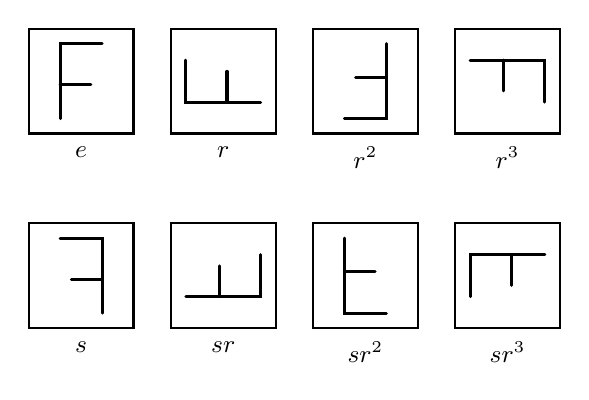
\begin{tikzpicture}[scale=0.95]
  \def\Fsym{\draw[line width=1.1pt, line cap=round]
      (-0.28,-0.5) -- (-0.28,0.5) -- (0.28,0.5)
      (-0.28,-0.05) -- (0.13,-0.05);}
  \foreach \ang/\lab [count=\i from 0] in {0/e, 90/r, 180/r^2, 270/r^3} {
    \begin{scope}[xshift=\i*1.9cm]
      \draw[thick] (0.05,0.05) rectangle (1.45,1.45);
      \begin{scope}[shift={(0.75,0.75)}]
        \begin{scope}[rotate=\ang]
          \Fsym
        \end{scope}
      \end{scope}
      \node[below, font=\small] at (0.75,0.0) {$\lab$};
    \end{scope}
  }
  \foreach \ang/\lab [count=\i from 0] in {0/s, 90/sr, 180/sr^2, 270/sr^3} {
    \begin{scope}[xshift=\i*1.9cm, yshift=-2.6cm]
      \draw[thick] (0.05,0.05) rectangle (1.45,1.45);
      \begin{scope}[shift={(0.75,0.75)}]
        \begin{scope}[xscale=-1]
          \begin{scope}[rotate=\ang]
            \Fsym
          \end{scope}
        \end{scope}
      \end{scope}
      \node[below, font=\small] at (0.75,0.0) {$\lab$};
    \end{scope}
  }
\end{tikzpicture}
\\[4pt]
{\small 图：正方形（$D_8$）的八个对称。上行为旋转 $e,r,r^2,r^3$；下行为反射 $s,sr,sr^2,sr^3$（分别关于四条对称轴，其中 $s$ 关于竖直轴）；$r$ 是逆时针转 $90^\circ$。}
\end{minipage}
\end{center}


用生成元和关系写成

\[D_{2n}=\langle r,s\mid r^n=s^2=e,\ rs=sr^{-1}\rangle.\]


\begin{center}
\begin{minipage}{0.95\textwidth}
\centering
\begin{tikzpicture}[scale=1.0]
  \draw[thick] (0:1.5) \foreach \a in {60,120,180,240,300} { -- (\a:1.5) } -- cycle;
  \foreach \a in {0,60,120,180,240,300} { \fill (\a:1.5) circle (1.5pt); }
  \draw[-{Stealth[length=2.5mm]}, thick] (5:1.75) arc (5:55:1.75);
  \node at (30:2.15) {$r$};
  \draw[dashed] (0,-1.9) -- (0,1.9);
  \node[above] at (0,1.9) {$s$};
\end{tikzpicture}
\\[4pt]
{\small 图：$D_{2n}$ 的生成元——旋转 $r$ 与关于竖直虚线轴的反射 $s$（图中 $n=6$）。}
\end{minipage}
\end{center}


由此可得 $r^ks=sr^{-k}$，于是每个元素都能唯一地写成

\[r^k\quad\text{或}\quad sr^k,\qquad 0\le k<n,\]

即 $D_{2n}=\{e,r,\ldots,r^{n-1},s,sr,\ldots,sr^{n-1}\}$。

例如

\[(sr^2)(sr^5)=s(r^2s)r^5=s(sr^{-2})r^5=r^3.\]

注意 $r^2s=sr^{-2}$，不能把 $r^2s$ 写成 $sr^2$。当 $n\ge3$ 时 $D_{2n}$ 一般不是 Abel 群，例如 $sr=r^{-1}s$。

\subsection{自由群}


给定字母表 $S$。把每个 $s\in S$ 与形式逆记号 $s^{-1}$ 放在一起，$S$ 上的词（word）是有限字符串

\[w=s_1^{\varepsilon_1}s_2^{\varepsilon_2}\cdots s_k^{\varepsilon_k},\qquad s_i\in S,\quad \varepsilon_i\in\{1,-1\},\]

空串（长度为 $0$ 的词，记作 $e$）也允许。

\textbf{相等关系。} 把能通过下面操作互相转化的词视为相等：在词中任意位置插入或删除相邻互逆对，

\[w\,ss^{-1}\,w'\sim w\,w',\qquad w\,s^{-1}s\,w'\sim w\,w'.\]

自由群（free group）$F(S)$ 的元素就是这些词模掉上述等价关系得到的等价类。

\textbf{群运算。} 两个类 $[u]$、$[v]$ 的乘积定义为：各取一个代表词 $u,v$，拼接起来，取拼接词所在的类，

\[[u]\cdot[v]=[uv].\]

换一组代表词不会改变结果：把 $u$ 换成同类词 $u'$，只需对拼接词 $uv$ 的前半段做同样的插入/删除，就得到 $u'v$，所以 $uv$ 与 $u'v$ 同类；对 $v$ 同理。因此乘法是良定义的。

例如 $[ab]\cdot[b^{-1}c]$：拼接得 $ab\,b^{-1}c$，删去 $bb^{-1}$ 得 $ac$，所以乘积是 $[ac]$。

空词的类 $e$ 是单位元。词 $w=s_1^{\varepsilon_1}\cdots s_k^{\varepsilon_k}$ 的逆元是反序并逐个取逆：

\[w^{-1}=s_k^{-\varepsilon_k}\cdots s_1^{-\varepsilon_1},\]

因为 $w\,w^{-1}=s_1^{\varepsilon_1}\cdots s_k^{\varepsilon_k}\,s_k^{-\varepsilon_k}\cdots s_1^{-\varepsilon_1}$ 中的互逆对可以逐对删去，最后剩下空词。

\textbf{自由性。} 自由群中除了由群的性质可推出相等的以外都不相等：例如 $aba^{-1}b^{-1}\ne e$，而 $abb^{-1}a^{-1}=e$。

\subsection{关系与表示}


$\langle r,s\mid r^n=s^2=e,\ rs=sr^{-1}\rangle$ 这种写法叫群的表示（presentation）：竖线左边是生成元（generators），右边是关系（relations）。

对照自由群：$F(r,s)$ 的相等最少——只承认由群的性质推出的相等；在它上面再要求 $r^n=e$、$s^2=e$、$rs=sr^{-1}$ 成立，能推出的相等变多，得到的群正是 $D_{2n}$。

有了关系就可以化简词，例如由 $rs=sr^{-1}$ 得 $r^ks=sr^{-k}$，于是每个元素都能整理成 $r^k$ 或 $sr^k$ 的形式。
